\usepackage{ctex} 
\usepackage{geometry,graphicx,color}
\geometry{
  a4paper,
  top=25.4mm, bottom=25.4mm,
  left=20mm, right=20mm,
  headheight=2.17cm,
  headsep=4mm,
  footskip=12mm
}
\usepackage[dvipsnames]{xcolor}
\usepackage{tikz}
\usetikzlibrary{backgrounds}
\usetikzlibrary{arrows,shapes}
\usetikzlibrary{tikzmark}
\usetikzlibrary{calc}
\usepackage{mathtools, nccmath}
\usepackage{comment}

% To generate dummy text
\usepackage{blindtext}

\usepackage{graphicx}
\usepackage{xspace}

% table alignment
\usepackage{array}
\usepackage{ragged2e}
\newcolumntype{P}[1]{>{\RaggedRight\hspace{0pt}}p{#1}}
\newcolumntype{X}[1]{>{\RaggedRight\hspace*{0pt}}p{#1}}

% color box
\usepackage{tcolorbox}


% for tikz
\usepackage{tikz}
\usetikzlibrary{arrows,shapes,positioning,shadows,trees,mindmap}
\usepackage[edges]{forest}
\usetikzlibrary{arrows.meta}
\colorlet{linecol}{black!75}
\usepackage{xkcdcolors} % xkcd colors


% for colorful equation
\usepackage{tikz}
\usetikzlibrary{backgrounds}
\usetikzlibrary{arrows,shapes}
\usetikzlibrary{tikzmark}
\usetikzlibrary{calc}
% Commands for Highlighting text -- non tikz method
\newcommand{\highlight}[2]{\colorbox{#1!17}{$\displaystyle #2$}}
\newcommand{\highlightdark}[2]{\colorbox{#1!47}{$\displaystyle #2$}}

% my custom colors for shading
\colorlet{mhpurple}{Plum!80}


% Commands for Highlighting text -- non tikz method
\renewcommand{\highlight}[2]{\colorbox{#1!17}{#2}}
\renewcommand{\highlightdark}[2]{\colorbox{#1!47}{#2}}

% Some math definitions
\newcommand{\lap}{\mathrm{Lap}}
\newcommand{\pr}{\mathrm{Pr}}

\newcommand{\Tset}{\mathcal{T}}
\newcommand{\Dset}{\mathcal{D}}
\newcommand{\Rbound}{\widetilde{\mathcal{R}}}

\usepackage[final]{pdfpages}
\usepackage{fontawesome5}
\usepackage{float}
\usepackage{wrapfig}
\usepackage{xchoices}
\usepackage{amssymb,amsmath,mathrsfs}        % 数学字体
\numberwithin{equation}{chapter}
\usepackage{unicode-math}
\setmathfont{texgyrepagella-math.otf}        % TeX Gyre Pagella 字体我的神
\usepackage{tgpagella}
\usepackage[T1]{fontenc}
\usepackage{fontspec}                        % 字体选择
\setmonofont{Consolas}                       % 设置无衬线字体为Consolas
\usepackage{paralist}
\usepackage{extarrows}
\let\itemize\compactitem
\let\enditemize\endcompactitem
\let\enumerate\compactenum
\let\endenumerate\endcompactenum
\let\description\compactdesc
\let\enddescription\endcompactdesc

\definecolor{winered}{rgb}{0.5,0,0}
\definecolor{structurecolor}{RGB}{122,122,142}
\definecolor{main}{HTML}{3D445F}
\definecolor{second}{HTML}{627581}
\definecolor{third}{HTML}{9D8798}

% 定义引用的颜色
\usepackage{hyperref}
\hypersetup{colorlinks = true, linktoc=all, linkcolor=winered, urlcolor=winered}

% ------------------------------------------------------------%
% 定义定理环境
\usepackage{amsthm}
\newtheoremstyle{defstyle}{3pt}{3pt}{}{-3pt}{\bfseries\color{main}}{}{0.5em}{【\thmname{#1} \thmnumber{#2}】 \thmnote{(#3)}}
\newtheoremstyle{thmstyle}{3pt}{3pt}{\kaishu}{-3pt}{\bfseries\color{second}}{}{0.5em}{【\thmname{#1} \thmnumber{#2}】 \thmnote{(#3)}}
\newtheoremstyle{prostyle}{3pt}{3pt}{\kaishu}{-3pt}{\bfseries\color{third}}{}{0.5em}{【\thmname{#1} \thmnumber{#2}】 \thmnote{(#3)}}

\theoremstyle{thmstyle} %theorem style
  \newtheorem{theorem}{定理}[chapter]
\theoremstyle{defstyle} % definition style
  \newtheorem{exercise}[theorem]{题}
  \newtheorem{definition}[theorem]{定义}
  \newtheorem{lemma}[theorem]{引理}
  \newtheorem{corollary}[theorem]{推论}
\theoremstyle{prostyle} % proposition style
  \newtheorem{proposition}[theorem]{命题}
  \newtheorem{remark}[theorem]{注}

\renewenvironment{proof}[1][证明]{\par\underline{\textbf{#1.}} \;\fangsong}{\qed\par}
\newenvironment{solution}{\par\noindent{\color{main}{\textbf{解.}}} \;\kaishu}{\qed\par}
\newcommand{\intro}[1]{\rightline{\parbox[t]{5cm}{\footnotesize \fangsong\quad\; #1 }}}
% ------------------------------------------------------------%
% ------------------------------------------------------------%
% 水印
%\usepackage{draftwatermark}         % 所有页加水印
%\usepackage[firstpage]{draftwatermark} % 只有第一页加水印
%\SetWatermarkText{\kaishu 核工A002班\; 张恺\; 2206114031}           % 设置水印内容
%\SetWatermarkText{\includegraphics{fig/texlion.png}}         % 设置水印logo
%\SetWatermarkLightness{0.9}             % 设置水印透明度 0-1
%\SetWatermarkScale{0.4}                   % 设置水印大小 0-1  

% 设置章形式
\usepackage{titlesec, titletoc}
\linespread{1.2} 				
\usepackage{fancyhdr}
\fancyhf{}
\renewcommand{\headrule}{\color{structurecolor}\hrule width\textwidth}
\pagestyle{fancy}
\renewcommand{\headrulewidth}{1pt}
\fancypagestyle{plain}{\renewcommand{\headrulewidth}{0pt}\fancyhf{}\renewcommand{\headrule}{}}

\fancyhead[c]{\color{structurecolor}\kaishu\rightmark}
\fancyfoot[c]{\color{structurecolor}\small\thepage}

\titleformat{\chapter}[display]{\Large}
{\color{structurecolor}\filleft
\parbox{1cm}{\vbox to 1.5cm{\vfill\hbox to 4cm{\hfill\Huge \bfseries \color{structurecolor}{Chapter} \thechapter \hfill}}}}
{1ex}
{\color{structurecolor} \titlerule[1.5pt]\Large\bfseries \filright \vspace*{1em}}
[\vspace*{1em} {\titlerule[1.5pt]}]

\titleformat{\section}[frame]{\normalfont\color{structurecolor}}{\footnotesize \enspace \large \textcolor{structurecolor}{\S \,\thesection}\enspace}{6pt}{\Large\filcenter \bf \kaishu }


\titleformat{\subsection}[hang]{\bfseries}{\large\bfseries\color{structurecolor}\thesubsection\enspace}{1pt}{\color{structurecolor}\large\bfseries\filright}

\titleformat{\subsubsection}[hang]{\bfseries}{\large\bfseries\color{structurecolor}\thesubsubsection\enspace}{1pt}{\color{structurecolor}\large\bfseries\filright}
% ------------------------------------------------------------%
% 设置封面
\usepackage{titling}
\renewcommand*{\maketitle}{
    \begin{titlepage}
    % \newgeometry{margin = 0in}
    % \parindent=0pt
    % 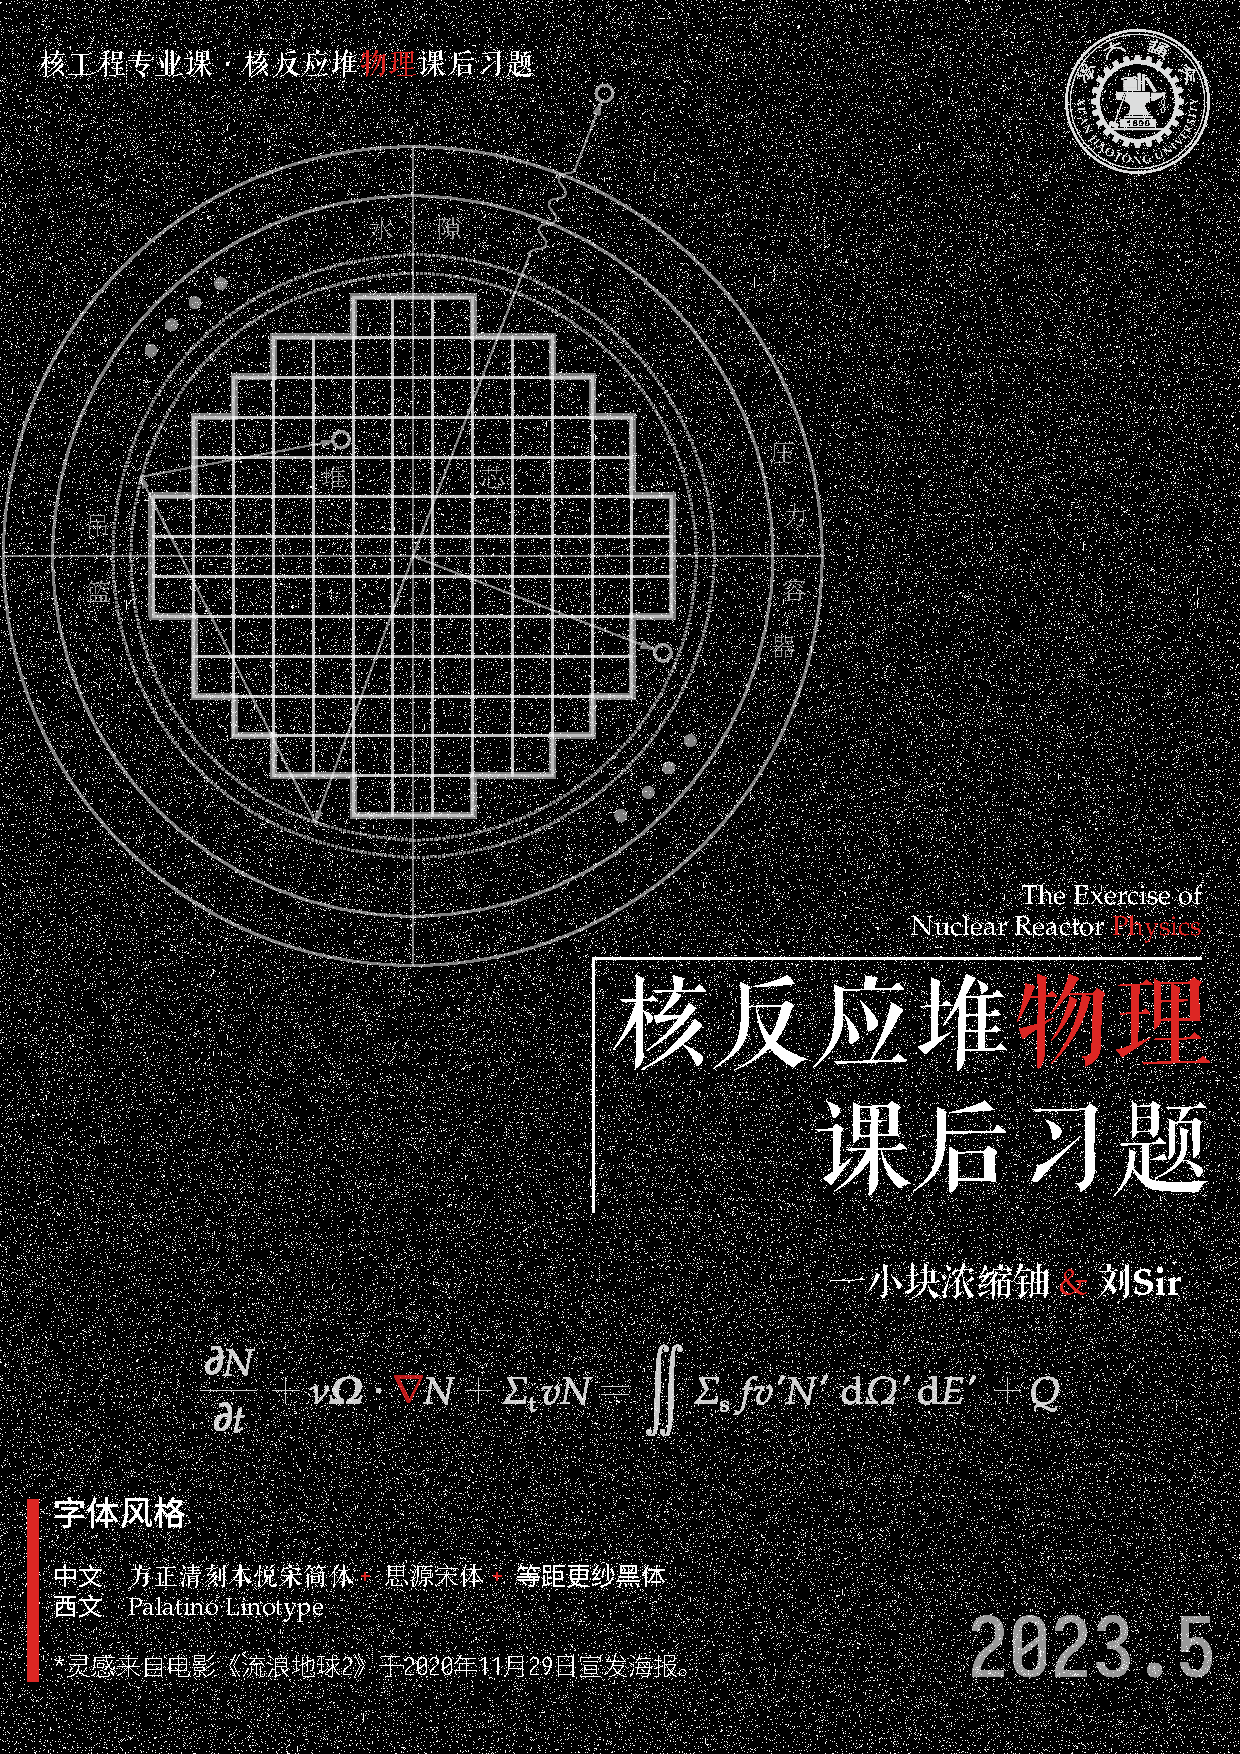
\includegraphics[width=\linewidth]{cover.jpg}
    % \vfill
    % \begin{center}
    %     \parbox{0.618\textwidth}{
    %     \hfill {\bfseries \Huge \thetitle} \\[0.6pt]  
    %     \rule{0.618\textwidth}{2pt} \\ 
    % }
    % \end{center}
    % \vfill
    % \begin{center}
    %     \parbox{0.618\textwidth}{
    %     \hfill\Large
    %     \kaishu 
    %       \begin{tabular}{r|}
    %       作者:\theauthor \\ 
    %       时间:\thedate \\
    %     \end{tabular}
    %     }
    % \end{center}
    % \vfill
    % \begin{center}
    %     \parbox[t]{0.7\textwidth}{\centering \kaishu }
    % \end{center}
    % \vfill
    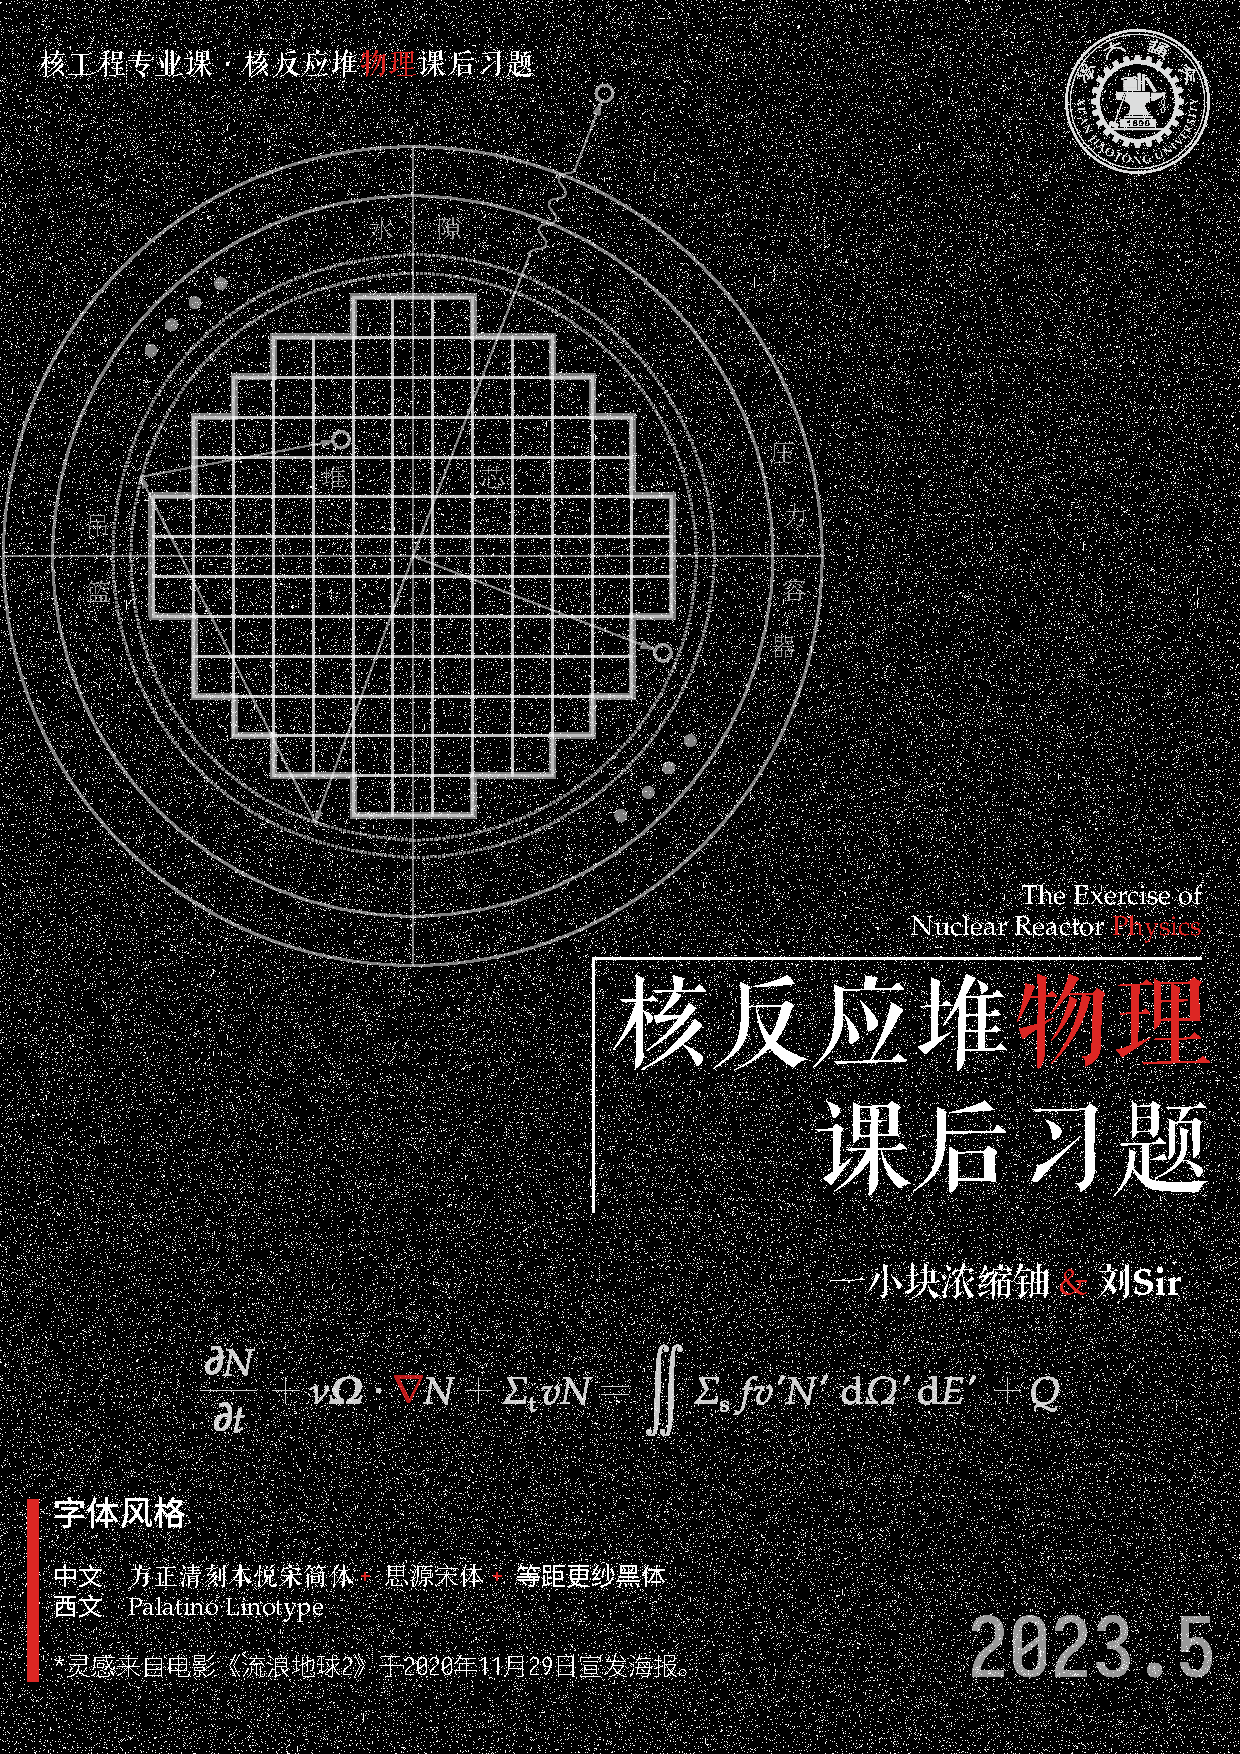
\includepdf{cover.pdf}
\end{titlepage}
}

\newcommand*{\keff}{k_{\symrm{eff}}}
\newcommand*{\dv}[2]{\frac{\symrm{d}{#1}}{\symrm{d}{#2}}}
\newcommand*{\ddv}[2]{\frac{\symrm{d^2}{#1}}{\symrm{d}{#2}^2}}
\newcommand*{\dd}[1]{\,\symrm{d}{#1}}
\newcommand*{\loge}{\symrm{ln}}
\newcommand*{\nsin}{\symrm{sin}}
\newcommand*{\ncos}{\symrm{cos}}
\newcommand*{\ntan}{\symrm{tan}}
\newcommand*{\vPhi}{\symit{\Phi}}
\newcommand*{\vSigma}{\symit{\Sigma}}
\newcommand*{\vLambda}{\symit{\Lambda}}
\newcommand*{\pddv}[2]{\frac{\symrm{\partial^2}{#1}}{\symrm{\partial}{#2}^2}}